% Exemplo de relatório técnico do IC

% Criado por P.J.de Rezende antes do Alvorecer da História.
% Modificado em 97-06-15 e 01-02-26 por J.Stolfi.
% modificado em 2003-06-07 21:12:18 por stolfi
% modificado em 2008-10-01 por cll
% \def\lastedit{2010-03-16 17:56:58 by stolfi}

\nonstopmode % PARA RODAR LATEX EM BATCH MODE
\documentclass[11pt,twoside]{article}

%INSERTED BY ME
%used to comment mutiple lines within a document
\usepackage{verbatim}
\usepackage[toc,page]{appendix}
\usepackage{float}
\usepackage{indentfirst} %indent all the paragrafers
\usepackage[pdftex]{hyperref}
\usepackage{listings}
\usepackage{color}
\renewcommand*{\lstlistingname}{C\'{o}digo}
\renewcommand{\lstlistlistingname}{Lista de C\'{o}digos}
\def\lstlistingautorefname{SQL Code}
\lstset{escapeinside=||}

\definecolor{dkgreen}{rgb}{0,0.6,0}
\definecolor{gray}{rgb}{0.5,0.5,0.5}
\definecolor{mauve}{rgb}{0.58,0,0.82}

\lstset{ %
  language=C,                % the language of the code
  basicstyle=\footnotesize,           % the size of the fonts that are used for the code
  numbers=left,                   % where to put the line-numbers
  numberstyle=\tiny\color{gray},  % the style that is used for the line-numbers
  stepnumber=2,                   % the step between two line-numbers. If it's 1, each line 
                                  % will be numbered
  numbersep=5pt,                  % how far the line-numbers are from the code
  backgroundcolor=\color{white},      % choose the background color. You must add \usepackage{color}
  showspaces=false,               % show spaces adding particular underscores
  showstringspaces=false,         % underline spaces within strings
  showtabs=false,                 % show tabs within strings adding particular underscores
  frame=single,                   % adds a frame around the code
  rulecolor=\color{black},        % if not set, the frame-color may be changed on line-breaks within not-black text (e.g. commens (green here))
  tabsize=2,                      % sets default tabsize to 2 spaces
  captionpos=b,                   % sets the caption-position to bottom
  breaklines=true,                % sets automatic line breaking
  breakatwhitespace=false,        % sets if automatic breaks should only happen at whitespace
  title=\lstname,                   % show the filename of files included with \lstinputlisting;
                                  % also try caption instead of title
  keywordstyle=\color{blue},          % keyword style
  commentstyle=\color{dkgreen},       % comment style
  stringstyle=\color{mauve},         % string literal style
}

\begin{comment}

    %--------------------------------SECTION{COMMENT}----------------------------------------
    
    \section{}
    
    %--------------------------------END{COMMENT}--------------------------------------------


    %--------------------------------SUBSECTION{COMMENT}-------------------------------------
        
        \subsection{}

    %--------------------------------END{COMMENT}--------------------------------------------

    %--------------------------------SUBSUBSECTION{COMMENT}----------------------------------
    
            \subsubsection{}
            
    %--------------------------------END{COMMENT}--------------------------------------------

% Inserting Image

    \begin{figure}[H]
        \centering
    	\includegraphics[width=11cm,height=8cm]{}
		\caption{}
		\label{}
	\end{figure}

% Inserting Code----------------------------

\usepackage{listings}
\usepackage{color}
\lstset{escapeinside=||}

\definecolor{dkgreen}{rgb}{0,0.6,0}
\definecolor{gray}{rgb}{0.5,0.5,0.5}
\definecolor{mauve}{rgb}{0.58,0,0.82}

\lstset{ %
  language=C,                % the language of the code
  basicstyle=\footnotesize,           % the size of the fonts that are used for the code
  numbers=left,                   % where to put the line-numbers
  numberstyle=\tiny\color{gray},  % the style that is used for the line-numbers
  stepnumber=2,                   % the step between two line-numbers. If it's 1, each line 
                                  % will be numbered
  numbersep=5pt,                  % how far the line-numbers are from the code
  backgroundcolor=\color{white},      % choose the background color. You must add \usepackage{color}
  showspaces=false,               % show spaces adding particular underscores
  showstringspaces=false,         % underline spaces within strings
  showtabs=false,                 % show tabs within strings adding particular underscores
  frame=single,                   % adds a frame around the code
  rulecolor=\color{black},        % if not set, the frame-color may be changed on line-breaks within not-black text (e.g. commens (green here))
  tabsize=2,                      % sets default tabsize to 2 spaces
  captionpos=b,                   % sets the caption-position to bottom
  breaklines=true,                % sets automatic line breaking
  breakatwhitespace=false,        % sets if automatic breaks should only happen at whitespace
  title=\lstname,                   % show the filename of files included with \lstinputlisting;
                                  % also try caption instead of title
  keywordstyle=\color{blue},          % keyword style
  commentstyle=\color{dkgreen},       % comment style
  stringstyle=\color{mauve},         % string literal style
}

% Enumerate with roman
\renewcommand{\theenumi}{\roman{enumi}}
\begin{enumerate}

\end{comment}
%INSERTED BY ME



\usepackage{techrep-ic}

%%% SE USAR INGLÊS, TROQUE AS ATIVAÇÕES DOS DOIS COMANDOS A SEGUIR:
\usepackage[brazil]{babel}
%% \usepackage[english]{babel}

%%% SE USAR CODIFICAÇÃO LATIN1 OU UTF-8, ATIVE UM DOS DOIS COMANDOS A
%%% SEGUIR:
%%\usepackage[latin1]{inputenc}
\usepackage[utf8]{inputenc}

%%% Para obter o tamanho de texto recomendado:
\usepackage[margin=1in]{geometry}


\begin{document}

%%% PÁGINA DE CAPA %%%%%%%%%%%%%%%%%%%%%%%%%%%%%%%%%%%%%%%%%%%%%%%
% 
% Número do relatório
\TRNumber{001}

% DATA DE PUBLICAÇÃO (PARA A CAPA)
%
\TRYear{14} % Dois dígitos
\TRMonth{3} % Numérico, 01-12

% LISTA DE AUTORES PARA CAPA (sem afiliações).
\TRAuthor{F. N. Candiani \and M. L. Junior \and R. H. F. Minami}

% TÍTULO PARA A CAPA (use \\ para forçar quebras de linha).
\TRTitle{Comparação de \textit{speedup} de\\ programas paralelos e sequenciais}

\TRMakeCover

%%%%%%%%%%%%%%%%%%%%%%%%%%%%%%%%%%%%%%%%%%%%%%%%%%%%%%%%%%%%%%%%%%%%%%
% O que segue é apenas uma sugestão - sinta-se à vontade para
% usar seu formato predileto, desde que as margens tenham pelo
% menos 25mm nos quatro lados, e o tamanho do fonte seja pelo menos
% 11pt. Certifique-se também de que o título e lista de autores
% estão reproduzidos na íntegra na página 1, a primeira depois da
% página de capa.
%%%%%%%%%%%%%%%%%%%%%%%%%%%%%%%%%%%%%%%%%%%%%%%%%%%%%%%%%%%%%%%%%%%%%%

%%%%%%%%%%%%%%%%%%%%%%%%%%%%%%%%%%%%%%%%%%%%%%%%%%%%%%%%%%%%%%%%%%%%%%
% Nomes de autores ABREVIADOS e titulo ABREVIADO,
% para cabeçalhos em cada página.
%
\markboth{Candiani, Junior e Minami}{Speedup paralelo e sequencial}
\pagestyle{myheadings}
\thispagestyle{empty}

%%%%%%%%%%%%%%%%%%%%%%%%%%%%%%%%%%%%%%%%%%%%%%%%%%%%%%%%%%%%%%%%%%%%%%
% TÍTULO e NOMES DOS AUTORES, completos, para a página 1.
% Use "\\" para quebrar linhas, "\and" para separar autores.
%
\title{Comparação de \textit{speedup} de programas paralelos e sequenciais}

\author{Fernando N. Candiani\thanks{Inst.~de Ciências Matemáticas e Computação, USP. N USP: 7239131 \texttt{fncandiani@usp.br}} \and
Marcius L. Junior\thanks{Inst.~de Ciências Matemáticas e Computação, USP. N USP: 7277433 \texttt{marcius@usp.br}} \and
Rafael H. F. Minami\thanks{Inst.~de Ciências Matemáticas e Computação, USP. N USP: 7573187 \texttt{rafahiroki@usp.br}}}

\date{}

\maketitle

%%%%%%%%%%%%%%%%%%%%%%%%%%%%%%%%%%%%%%%%%%%%%%%%%%%%%%%%%%%%%%%%%%%%%%

\tableofcontents
\listoffigures
\listoftables
\lstlistoflistings

\clearpage

\begin{abstract} 
    In this assignment we used the Monte Carlo simulation to calculate the $\pi$ number and
    also the Black Scholes model. In each case, we build an program that use different
    programming paradigms; one sequencial and the other parallel. After executing each
    program multiples times we calculated the speedup so we could compare the improvement
    of the usage of parallel paradigm rather than sequencial. This article shows the results
    obtained during the experiments and problems regarding the implementation of the 
    parallel algorithm and its execution.
\end{abstract}


\section{Introdução}

    Nesse trabalho utilizamos a simulação de Monte Carlo para calcular o número $\pi$ e 
    também o modelo de Black-Scholes. Foram desenvolvidas duas versões de
    cada algoritmo, uma sequencial e outra paralela utilizando \textit{threads}. Neste relatório
    nós mostraremos os resultados obtidos e faremos a comparação entre a versão sequencial e a
    paralela dos dois algoritmos. Todos os códigos e saídas dos programas, bem como os métodos
    de compilação, podem ser encontrados dentro do nosso repositório do 
    {\it Google Code}\footnote{https://code.google.com/p/pc2014-grupo09-turmab/\label{fnt:code}}.

    \subsection{Monte Carlo}
    
        Definimos por um método de Monte Carlo (MMC), um método qualquer de uma classe
        de método estatísticos, que inferem de amostragens massivas para obter resultados
        numéricos, isto é, repetem exaustivamente simulações, afim de calcular probabilidades
        heuristicamente, tal com se, de fato, se registrassem os resultado reais de jogos em
        cassino, da onde derivou-se o nome.
    
        Apesar de ter se despertado o interesse por esse método durante a Segunda Guerra
        Mundial, na construção de uma bomba atômica, quando foi batizado com o nome. A
        técnica de Monte Carlo já era utilizada em uma discussão das equações de Boltzmann,
        onde é calculado a função de distribuição de partículas em estados diferente.
        
    %Designa-se por método de Monte Carlo (MMC) qualquer método de uma classe de métodos estatísticos que se baseiam em amostragens aleatórias massivas para obter resultados numéricos, isto é, repetindo sucessivas simulações um elevado numero de vezes, para calcular probabilidades heuristicamente, tal como se, de facto, se registassem os resultados reais em jogos de casino (daí o nome). 
    %De acordo com (HAMMERSELEY,1964) o nome "Monte Carlo" surgiu durante o projeto Manhattan na Segunda Guerra Mundial. No projeto de construção da bomba atómica, Ulam, von Neumann e Fermi consideraram a possibilidade de utilizar o método, que envolvia a simulação direta de problemas de natureza probabilística relacionados com o coeficiente de difusão do neutron em certos materiais. Apesar de ter despertado a atenção desses cientistas em 1948, a lógica do método já era conhecida há bastante tempo. Por exemplo, existe um registro de um artigo escrito por Lord Kelvin dezenas de anos antes, que já utilizava técnicas de Monte Carlo em uma discussão das equações de Boltzmann.
    
    \subsection{Black-Scholes}
    
        A fórmula de Black-Scholes for apresentada inicialmente em \cite{BS}. A base para sua
        pesquisa utilizou o trabalho desenvolvido por pesquisadores como Jack L. Treynor, Paul
        Samuelson, A. James Boness, Sheen T. Kassouf, e Edward O. Thorp. O conceito fundamental
        de {\it Black-Scholes} é que se uma ação é negociada, então a opção é precificada.
            
        Conforme mostrado em \cite{M} Robert C. Merton foi o primeiro a mostrar uma expansão da
        compreensão matemática do modelo de precificação de opções, e cunhou o termo modelo de
        precificação de opções de {\it Black-Scholes}.

\section{Método Monte Carlo para cálculo de $\pi$}

    Uma simplificação do algoritmo de Metropolis utilizamos o Monte Carlo de Erro-Unilateral
    para calcular a aproximação de $\pi$, que consiste em uma distribuição amostral onde o 
    evento não pertence é garantida a resposta - garantimos que o ponto que não pertencem ao
    círculo, com certeza se encontram no quadrado; porém quando o amostra pertence não é 
    garantida que a resposta esta correta - temos de verificar se cada conjunto de coordenadas
    se encontra no interior do círculo.

    \subsection{Algoritmo}
        
        Neste algoritmo, para utilizar o método de Monte Carlo nós consideramos uma circunferência
        inscrita em um quadrado. A relação entre as áreas é $\frac{\pi}{4}$ e por isso nós
        conseguimos chegar ao valor de $\pi$ utilizando o método de Monte Carlo.
        
        Utilizando uma função que gera números randômicos, conseguimos escolher pontos 
        aleatórios dentro desse quadrado. No fim teremos o número de pontos que estão dentro
        da circunferência e o número total de pontos gerados. Figura \ref{img:montecarlo}
        
        A razão entre os dois números é uma aproximação da razão das duas áreas que é
        $\frac{\pi}{4}$, portanto, devemos multiplicar essa razão por $4$ e assim teremos
        uma aproximação do número $\pi$.

        \begin{figure}[H]
            \centering
        	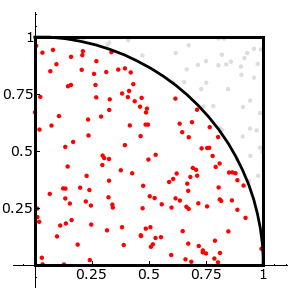
\includegraphics[scale=0.8]{figures/monte_carlo.png}
    		\caption{Método de Monte Carlo aplicado para encontrar o valor aproximado de $\pi$}
    		\label{img:montecarlo}
    	\end{figure}
	
        Fizemos duas versões desse algoritmo, uma totalmente sequencial e outra paralela
        utilizando \textit{threads}. Na versão com \textit{threads} tivemos que observar
        o que poderia ser paralelizado. A maneira que encontramos foi paralelizar o laço
        que gera os pontos aleatórios.

    \subsection{Como rodar o programa}
    
        Nesta seção é apresentado como é feita a compilação e execução e os parâmetros de execução
        e, também, os de entrada do programa.
    
        \subsubsection{Sequencial}
        
            Estando dentro do diretório {\it montecarlo/sequencial} onde contém os arquivos
            {\it makefile} e {\it montecarlo.c}, que pode ser visto em Código
            \ref{code:montecarlo_seq}, devemos executar os seguintes comandos:\\
        
            {\it usuer@pc-name:dir~\$ make}\\
            
            O comando {\it make} irá compilar o Código \ref{code:montecarlo_seq} passando
            todos os parâmetros de lincagem das bibliotecas extras.\\
            
            {\it user}@{\it pc-name:dir~}\${\it /usr/bin/time -f }"\%{\it e}" ./{\it montecarlo}
            $>>$ {\it path}/{\it file.out 2}$>$\&{\it 1} \\
            
            O comando irá executar o programa para o cálculo de $\pi$, redirecionando o tempo
            e o valor de $\pi$ para {\it file.out}.\\
        
        \subsubsection{Paralelo}
        
            Estando dentro do diretório {\it montecarlos/paralelo} onde contém os arquivos 
            {\it makefile} e {\it montecarlo.c}, que pode ser visto em Código 
            \ref{code:montecarlo_par}, devemos executar os seguintes comandos:\\
            
            {\it usuer@pc-name:dir~\$ make}\\
            
            O comando {\it make} irá compilar o Código \ref{code:montecarlo_par}
            passando todos os parâmetros de lincagem das bibliotecas extras.\\
                
            {\it user}@{\it pc-name:dir~}\${\it /usr/bin/time -f }"\%{\it e}" ./{\it montecarlo}
            [{\it number of threads}] $>>$ {\it path}/{\it file.out 2}$>$\&{\it 1}\\
            
            O comando irá executar o programa para o cálculo do valor de $\pi$, recebendo como 
            parâmetro o {\it number of threads} e redirecionando o tempo e o valor de $\pi$
            para {\it file.out}.


    \subsection{Dificuldades e Soluções}
    
        Para o problema sequencial tivemos uma dificuldade para entender o funcionamento da
        função {\it double erand48(unsigned short xsubi[3])} pois essa recebe um parâmetro que
        serve como seed para os valores randômicos que serão gerados posteriormente dentro da
        função, ou seja, os valores do vetor {\it xsubi} eram, inicialmente, inicializados com
        um valor constante e a cada execução do programa a saída dos valores randômicos
        eram sempre as mesmas. Para solucionar esse problema foi utilizado a função
        {\it time(NULL)} nas posições 1 e 2 do vetor {\it xsubi}. Posteriormente, a função
        foi mudada para a {\it double drand48(void)} pois esta é {\it thread-safe} e para
        inicializar a semente da função randômica utilizamos a função
        {\it void srand48(long int seedval)}.
        
        Para o problema paralelo tivemos problema na modelagem da solução, ou seja, como
        iriamos resolver o problema de forma paralelizada. A solução foi discutida entre
        colegas na sala e conseguimos extrair um modelo que, inclusive, foi posteriormente
        discutido em sala. A solução envolvia um vetor global com o tamanho do número de
        {\it threads} em que o programa vai ser separado, ou seja, em um programa que tem 16
        {\it threads} teríamos um vetor com tamanho 16. E em cada posição do vetor a sua
        {\it thread} correspondente irá atualizar o número de acertos que ocorreu, entenda
        acertos como pontos $(x,y)$ que estão dentro da circunferência de raio igual a 1.

    \subsection{Resultados Obtidos}
    
        Por se tratar de um problema em que o número de interações é muito grande, que 
        em nosso caso é definido como um parâmetro $10^9$, o tempo de execução sempre é 
        razoalmente grande, conforme pode ser visto dentro das saídas geradas dentro do
        repositório do {\it Google Code} \ref{fnt:code}.
        
        Para os programas sequencial e paralelo os dados obtidos são apresentados na Tabela 
        \ref{tab:montecarlo_seq} e Tabela \ref{tab:montecarlo_par}, respectivamente.
        
        \begin{table}[ht]
        \centering
            \begin{tabular}{|c|c|c|}
             \hline
            & Média & Variância \\ \hline
            $\pi$ & 3.141578 & 0.000000 \\ \hline
            Tempo & 39.735000 & 0.048050 \\ \hline
            \end{tabular}
        \caption{Média e Variância para os dados do {\it Monte Carlo} sequencial.}
        \label{tab:montecarlo_seq}
        \end{table}
        
        \begin{figure}[ht]
            \centering
        	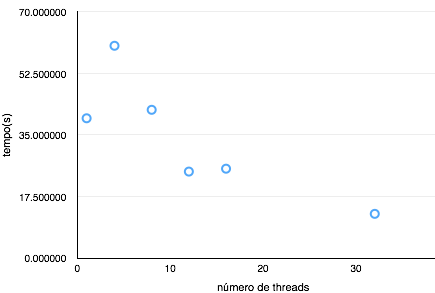
\includegraphics[scale=0.8]{figures/grafico_montecarlo.png}
    		\caption{Gráfico {\it threads} x tempo(s) para o algoritmo de cálculo de $\pi$.}
    		\label{img:grafico_montecarlo}
    	\end{figure}
    	
        \begin{table}[ht]
        \centering
            \begin{tabular}{|c|c|c|}
            \hline
            
            \multicolumn{3}{|c|}{ 4 {\it Threads} } \\ \hline
            
             & Média & Variância \\ \hline
             $\pi$ & 3.141586 & 0.000000 \\ \hline
            Tempo & 60.325427 & 1.015872 \\ \hline
            
            \multicolumn{3}{|c|}{ 8 {\it Threads} } \\ \hline
            
             & Média & Variância \\ \hline
            $\pi$ & 3.141592 & 0.000000 \\ \hline
            Tempo & 42.139608 & 4.870509 \\ \hline
            
            \multicolumn{3}{|c|}{ 12 {\it Threads} } \\ \hline
            
             & Média & Variância \\ \hline
             $\pi$ & 3.141586 & 0.000000 \\ \hline
            Tempo & 24.598560 & 0.660768 \\ \hline
            
            \multicolumn{3}{|c|}{ 16 {\it Threads} } \\ \hline
            
             & Média & Variância \\ \hline
            $\pi$ & 3.141588 & 0.000000 \\ \hline
            Tempo & 25.417140 & 0.785086 \\ \hline
            
            \multicolumn{3}{|c|}{ 32 {\it Threads} } \\ \hline
            
             & Média & Variância \\ \hline
             $\pi$ & 3.141588 & 0.000000 \\ \hline
            Tempo & 12.595500 & 0.146668 \\ \hline
            
            
            \end{tabular}
        \caption{Média e Variância para os dados do {\it Monte Carlo} paralelo.}
        \label{tab:montecarlo_par}
        \end{table}
    
    
        Conforme pode ser visto, tanto nas Tabelas \ref{tab:montecarlo_seq} e
        \ref{tab:montecarlo_par} quanto na Figura \ref{img:grafico_montecarlo}, houve
        uma diminuição considerável no tempo de execução entre o programa sequêncial e
        paralelo, apenas para um número de threads maior que $8$, exclusive.
        O {\it speedup} para $4$ e $8$ {\it threads} foi $< 1$ o que representa um
        aumento no tempo de execução do programa paralelo em relação ao sequencial. Isso,
        possivelmente, se deve ao fato de o algoritmo paralelo adicionar complexidade
        de memória, ou seja, dentro do Código \ref{code:montecarlo_par} podemos ver
        que foi adicionado muito mais alocação de memório em relação ao Código
        \ref{code:montecarlo_seq}, o que fez ocorrer o aumento de operação de memória
        e por consequência o tempo de execução do programa.
        
        Para $12$ e $16$ {\it threads}, o {\it speedup } calculado ficou em torno de
        $1.61$, ou seja, o programa paralelo foi cerca de $1.61$ vezes mais rápido
        que o sequencial, o que representa um aumento
        razoavelmente bom para o tempo de execução. Já para $32$ {\it threads} o {\it speedup}
        calculado foi $3,15$, o que representa um aumento muito considerável, para entender o
        cálculo do {\it speedup} consulte a Seção \ref{sec:speedup}.

\section{Modelo de Black-Scholes}

    O modelo de Black-Scholes do mercado para um ativo faz as seguintes suposições explícitas:
    
    \begin{enumerate}
        \item É possível emprestar e tomar emprestado a uma taxa de juros livre de risco
            constante e conhecida;
        \item O preço segue um movimento Browniano geométrico com tendência (drift) e 
            volatilidade constantes;
        \item Não há custos de transação;
        \item A ação não paga dividendos;
        \item Não há restrições para a venda a descoberto.
    \end{enumerate}

    \subsection{Algoritmo}
    
        Para o modelo de Black-Scholes nós seguimos o algoritmo apresentado na Figura
        \ref{img:blackscholes}. Este algoritmo utiliza o método de
        Monte Carlo para calcular o preço das opções européias. As variáveis de entrada desse
        algoritmo são: 
        
        S: valor da ação,
        E: preço de exercício da opção,
        r: taxa de juros livre de risco (SELIC),
        $\sigma$: volatilidade da ação,
        T : tempo de validade da opção e 
        M : número de iterações.
    
        \begin{figure}[H]
            \centering
        	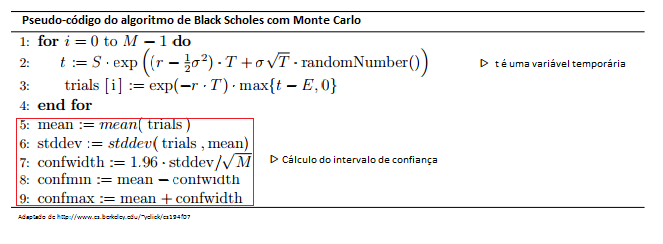
\includegraphics[scale=0.6]{figures/blackscholes.png}
    		\caption{Algoritmo do modelo de Black Scholes}
    		\label{img:blackscholes}
    	\end{figure}

\subsection{Como rodar o programa}
    
    Nesta seção é apresentado como é feita a compilação e execução e os parâmetros de execução
    e, também, os de entrada do programa.
    
    \subsubsection{Sequencial}
        Estando dentro do diretório {\it blackscholes/sequencial} onde contem os
        arquivos {\it makefile} e {\it blackscholes.c}, conforme pode ser visto em
        Código \ref{code:blackscholes_seq}, devemos executar os seguintes comandos:\\
        
        {\it usuer@pc-name:dir~\$ make}\\
        O comando {\it make} irá compilar o Código \ref{code:blackscholes_seq} passando
        todos os parâmetros de lincagem das bibliotecas extras.\\
            
        {\it user}@{\it pc-name:dir~}\${\it /usr/bin/time -f }"\%{\it e}" ./{\it blackshcoles}
        $<$ {\it file.in} $>>$ {\it path}/{\it file.out 2}$>$\&{\it 1}\\
        
            O comando irá executar o programa para cálculo de aproximação de valor confiável
            para aplicação de investimentos, recebendo a entra a de {\it file.in}, 
            redirecionando o tempo e as saídas do programa para {\it file.out}.
        
    \subsubsection{Paralelo}
        Estando dentro do diretório {\it blachsholes/paralelo} onde contem os arquivos
        {\it makefile} e {\it blackshcoles.c}, conforme pode ser visto em Código
        \ref{code:blackscholes_par}, devemos executar os seguintes comandos:\\
        
        {\it usuer@pc-name:dir~\$ make}\\
        
        O comando {\it make} irá compilar o Código \ref{code:blackscholes_par} passando
        todos os parâmetros de lincagem das bibliotecas extras.\\
            
        {\it user}@{\it pc-name:dir~}\${\it /usr/bin/time -f }"\%{\it e}" ./{\it blackshcoles} [{\it numeber of threads}] $<$ {\it file.in} $>>$ {\it path}/{\it file.out 2}$>$\&{\it 1}\\
        O comando irá executar o programa para cálculo de aproximação de valor confiável
        para aplicação de investimentos, recebendo como parâmetro o {\it  number of threads}
        e na entrada padrão o arquivo {\it file.in}, redirecionando o tempo e as saídas do
        programa para {\it file.out}.

    \subsection{Dificuldades e Soluções}
    
        O maior problema encontrado dentro do modelo de Black-Scholes foi a distribuição
        dos números randômicos. Os números randômicos desse modelo devem seguir uma distribuição 
        normal e não uma distribuição uniforme conforme exigido no cálculo de $\pi$. Com
        isso muitos problemas surgiram na hora de verificar se a solução aplicada estava
        correta.
        
        Tanto no desenvolvimento do programa sequencial quanto do programa paralelo
        não houve nenhum problema pois já estávamos habituados com a forma de pensamento
        para solucionar o problema.

    \subsection{Resultados Obtidos}

        Por se tratar de um problema em que o número de interações não é muito grande, que 
        em nosso caso é recebido como um parâmetro {\it M}, girando em torno, na grande maioria
        das vezes, de $1000$ a $5000$ iterações, o tempo de execução sempre é pequeno,
        conforme pode ser visto dentro das saídas geradas dentro do repositório do {\it Google
        Code} \ref{fnt:code}.
        
        Para os programas sequencial e paralelo os dados obtidos são apresentados na Tabela 
        \ref{tab:blackscholes_seq} e Tabela \ref{tab:blackscholes_par}, respectivamente.
        
        \begin{table}[ht]
        \centering
            \begin{tabular}{|c|c|c|}
             \hline
            & Média & Variância \\ \hline
            Média Calculada & 99.904995 & 0.000000 \\ \hline
            Intervalo de confiança & 0.793321 & 0.000000\\ \hline
            Tempo & 0.020920 & 0.000015 \\ \hline
            \end{tabular}
        \caption{Média e Variância para os dados do {\it Black-Scholes} sequencial.}
        \label{tab:blackscholes_seq}
        \end{table}

        \begin{table}[ht]
        \centering
            \begin{tabular}{|c|c|c|}
            \hline
            
            \multicolumn{3}{|c|}{ 4 {\it Threads} } \\ \hline
            
             & Média & Variância \\ \hline
            Média Calculada & 104.134842 & 0.030029 \\ \hline
            Intervalo de confiança & 0.184846 & 0.000000\\ \hline
            Tempo & 0.010010 & 0.000000 \\ \hline
            
            \multicolumn{3}{|c|}{ 8 {\it Threads} } \\ \hline
            
             & Média & Variância \\ \hline
            Média Calculada & 104.167049 & 0.052991 \\ \hline
            Intervalo de confiança & 0.184623 & 0.000000\\ \hline
            Tempo & 0.009520 & 0.000005 \\ \hline
            
            \multicolumn{3}{|c|}{ 12 {\it Threads} } \\ \hline
            
             & Média & Variância \\ \hline
            Média Calculada & 104.113276 & 0.127136 \\ \hline
            Intervalo de confiança & 0.185021 & 0.000001\\ \hline
            Tempo & 0.009040 & 0.000009 \\ \hline
            
            \multicolumn{3}{|c|}{ 16 {\it Threads} } \\ \hline
            
             & Média & Variância \\ \hline
            Média Calculada & 104.288167 & 0.077040 \\ \hline
            Intervalo de confiança & 0.185034 & 0.000001\\ \hline
            Tempo & 0.009330 & 0.000006 \\ \hline
            
            \multicolumn{3}{|c|}{ 32 {\it Threads} } \\ \hline
            
             & Média & Variância \\ \hline
            Média Calculada & 104.076457 & 0.225480 \\ \hline
            Intervalo de confiança & 0.185103 & 0.000003\\ \hline
            Tempo & 0.010000 & 0.000000 \\ \hline
            
            
            \end{tabular}
        \caption{Média e Variância para os dados do {\it Black-Scholes} paralelo.}
        \label{tab:blackscholes_par}
        \end{table}
        
        \begin{figure}[ht]
            \centering
        	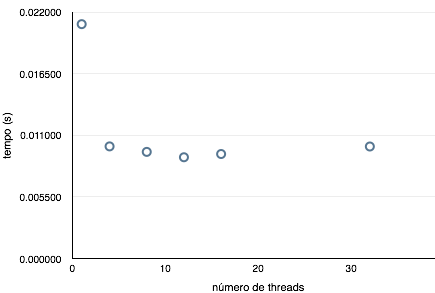
\includegraphics[scale=0.8]{figures/grafico_blackscholes.png}
    		\caption{Gráfico {\it threads} x tempo(s) para o algoritmo de {\it Black-Scholes}.}
    		\label{img:grafico_blackscholes}
    	\end{figure}
       
        Conforme pode ser visto, tanto nas Tabelas \ref{tab:blackscholes_seq} e
        \ref{tab:blackscholes_par} quanto na Figura \ref{img:grafico_blackscholes}, houve
        uma diminuição considerável no tempo de execução entre o programa sequêncial e paralelo.
        O {\it speedup } calculado ficou em torno de $2$, ou seja, o programa paralelo
        foi cerca de $2$ vezes mais rápido que o sequencial, o que representa um aumento
        considerável para o tempo de execução, para entender o cálculo do speedup
        consulte a Seção \ref{sec:speedup}.
        
        Podemos observar também pela Figura \ref{img:grafico_blackscholes} que um aumento
        no número de {\it threads} não significa um aumento de eficiência visto que está
        limitado ao número de núcleos que o hardware possui, pois quanto mais {\it threads},
        maior é o número de chaveamentos que ele deve fazer, portanto existe um ponto máximo
        em que se tem um ganho real, depois disso o tempo de chaveamento é grande e a 
        eficiência do programa é afetada.

\section{Metodologia de execução dos experimentos}

    Para a execução dos programas feitos, foi criado um \textit{script}, mostrado em Código
    \ref{code:script}, que é capaz de rodar todos os programas definidos (Monte Carlo -
    sequencial e paralelo, Black-Scholes - sequencial e paralelo) e para cada programa paralelo
    o \textit{script} altera o número de \textit{threads} que este vai executar.
    
    Esse \textit{script} faz a compilação e execução dos programas e após a execução esse
    redireciona todos os resultados para um arquivo. Esse arquivo, que foi formatado de forma
    simples, é utilizado para o cálculo da média e variância, conforme mostrado na
    Seção \ref{sec:mean_var}, dos dados que foram gerados pelos programas, assim podemos analisar
    melhor os resultados gerados.
    
    \subsection{Dificuldades e Soluções}

        Durante a execução do \textit{script} tivemos alguns problemas na conexão com o cluster
        gerando \textit{broken pipes} com este. Por isso, tivemos que fazer algumas alterações na
        chamada dos métodos criados dentro do \textit{script}, por exemplo, quando estavamos
        executando o Monte Carlo paralelo ocorreu um problema de conexão e tivemos que comentar
        a chamada de função do Monte Carlo sequencial pois este já havia sido executado.
        
        Outro problema gerado pela falha na conexão foi que o arquivo já possuía dados gerados
        na execução anterior e por isso o tipo de \textit{pipe}, que antes era um \textit{pipe}
        de redirecionamento simples, foi alterado para um \textit{pipe} de concatenação para que
        os dados gerados na execução anterior fossem mantidos e não fosse necessário a execução
        do \textit{script} desde do início.
        
        Outra problema encontrado no desenvolvimento do \textit{script} foi o redirecionamento
        da saída do programa \textit{/usr/bin/time} pois este redireciona sua saída para a
        \textit{stderr} ao invés da \textit{stdout}. A solução encontrada foi acrescentar
        uma \textit{flag} ao redirecionamento que faz com que o \textit{stderr} também seja redirecionado
        ao arquivo passado, isso foi obtido com o comando "2$>$\&1".
    

\section{Cálculo da média e da variância dos dados}
\label{sec:mean_var}

    Como a execução de cada programa foi feita múltiplas vezes, no nosso caso foi executado
    $1000$ vezes, seria inviável calcular a média e o desvio padrão dos dados gerados de forma
    manual. Por isso, foi criado um programa, conforme mostrado em Código \ref{code:mean_var},
    que dado o tamanho de um vetor e o número de variáveis a ser analisado calculará a média
    e variância, levando em consideração que os dados estão distribuídos da seguinte maneira:
    
    \ \\
    \ \indent quantidade dos dados \indent número de variáveis\\
    \ \indent dado 1 da variável a\\
    \ \indent dado 1 da variável b\\
    \ \indent dado 2 da variável a\\
    \ \indent dado 2 da variável b\\
    \ \indent e assim por diante.
    \ \\
    
    Os dados gerados por esse programa serão apresentados dentro das seções respectivas aos
    seus dados.

\section{Como calcular o {\it Speedup }}
\label{sec:speedup}

    Como o próprio termo já diz, o {\it speedup} é o ganho na velocidade quando se compara duas
    situações. No nosso caso usamos o {\it speedup} para calcular o ganho na velocidade de
    execução entre um programa sequencial e um programa paralelo, por isso para saber qual
    a vantagem entre os dois devemos resolver a seguinte razão:
    
    \begin{equation}
        S_p = \frac{T_1}{T_p}
    \end{equation}

    onde $S_p$ é o {\it speedup},
    
    $T_1$ é o tempo médio do algoritmo sequencial e
    
    $T_p$ é o tempo médio do algoritmo paralelo.\\
    
    Espera-se que esse número seja sempre $> 1$ pois isso mostra que o houve um ganho
    no algoritmo paralelo em relação ao sequencial. Para ter um bom {\it speedup}
    o valor $S_p$ esperado deve ser $ > 2$, ou seja, houve uma diminuição de cerca de
    $50\%$ no tempo de execução do programa sequencial em relação ao paralelo.

\section{Hardware utilizado}

    Para todos os programas o mesmo hardware foi utilizado, o do \textit{cluster}. Para obter
    a descrição detalhada do hardware utilizamos o seguinte programa, com um parâmetro:
    
    \ \\ \ \indent {\it phoronix-test-suite detailed-system-info}
    \ \\
    
    A saída obtida foi a seguinte (a grande maioria dos dados são auto-explicativos e por isso
    não será discutido):
    \ \\ \ \\
    {\hspace{2 cm}{\it Phoronix Test Suite v4.8.2\\
         System Information\\
        \ \\
        Hardware: \\
        Processor: Intel Core 2 Quad Q9400 @ 2.67GHz (4 Cores), \\
        Motherboard: Gigabyte G41MT-S2P,\\
        Chipset: Intel 4 DRAM + ICH7,\\
        Memory: 8192MB,\\
        Disk: 500GB Western Digital WD5000AACS-0,\\
        Graphics: Intel 4 IGP,\\
        Audio: VIA VT2020,\\
        Network: Realtek RTL8111/8168/8411
        \ \\
        Software:\\
        OS: Ubuntu 12.04, Kernel: 3.2.0-54-generic (x86\_64), Compiler: GCC 4.6,\\
        File-System: ext4, Screen Resolution: 640x480\\
        \ \\
        Processor: \\
        Core Count: 4\\
        Thread Count: 4\\
        Cache Size: 3072 KB\\
        Instruction Set Extensions: SSE 4.1\\
        AES Encryption: NO\\
        Energy Performance Bias: NO\\
        Virtualization: VT-x\\
        Compiler Configuration: --build=x86\_64-linux-gnu --disable-werror --enable-checking=release --enable-clocale=gnu --enable-gnu-unique-object --enable-languages=c,c++,fortran,objc,obj-c++ --enable-libstdcxx-debug --enable-libstdcxx-time=yes --enable-nls --enable-objc-gc --enable-plugin --enable six --host=x86\_64-linux-gnu --target=x86\_64-linux-gnu --with-arch-32=i686 --with-tune=generic -v\\
        Disk Scheduler: CFQ\\
        Disk Mount Options: barrier=1,data=ordered,relatime,rw,user\_xattr\\
        Cpu Scaling Governor: acpi-cpufreq ondemand}}

\section{Conclusão}

    A partir dos resultados obtidos através de nossos algoritmos fica clara a vantagem
    de se paralelizar processos para se obter um ganho considerável de eficiência. Em
    nossos testes também observamos que existe uma relação entre o número de núcleos
    que o hardware possui e o número máximo de threads que ele pode suportar, depois
    desse número máximo a eficiência é diminuída. Isso ocorre por causa da quantidade
    de chaveamentos que precisam ocorrer para que as {\it threads} executem, aumentando,
    assim, o tempo de execução.

\clearpage

\begin{appendices}

    \chapter{Script para execução dos experimentos}
        \lstinputlisting[caption=Script para execução dos experimentos, language=sh, label=code:script]{codes/script.sh}

    \ \\

    \chapter{Código para cálculo da média e variância dos dados}
        \lstinputlisting[caption=Cálculo da média e variância dos dados., label=code:mean_var]{codes/mean_var.c}
        
    \ \\
        
    \chapter{Código para cálculo de PI, usando método de Monte Carlo, algoritmo sequencial}
        \lstinputlisting[caption=Método de Monte Carlo sequencial., label=code:montecarlo_seq]{codes/montecarlo_seq.c}
        
    \ \\
        
    \chapter{Código para cálculo de PI, usando método de Monte Carlo, algoritmo usando paradigma de paralelismo}
        \lstinputlisting[caption=Método de Monte Carlo paralelo., label=code:montecarlo_par]{codes/montecarlo_par.c}
        
    \ \\
        
    \chapter{Código para cálculo de aproximação de valor confiável para aplicação de investimentos, usando método de Black-Scholes, algoritmo sequencial}
        \lstinputlisting[caption=Método de Black-Scholes sequencial., label=code:blackscholes_seq]{codes/blackscholes_seq.c}
        
    \ \\
        
    \chapter{Código para cálculo de aproximação de valor confiável para aplicação de investimentos, usando método de Black-Scholes, algoritmo usando paradigma de paralelismo}
        \lstinputlisting[caption=Método de Black-Scholes paralelo., label=code:blackscholes_par]{codes/blackscholes_par.c}
        
    \ \\

\end{appendices}

\clearpage

\begin{thebibliography}{99}

    \bibitem{BS} Black, Fischer; Myron Scholes. (1973). {\it The Pricing of Options and Corporate Liabilities}. Journal of Political Economy {\bf 81} (Black and Scholes' original paper.)
    
    \bibitem{M} Merton, Robert C.. (1973). {\it Theory of Rational Option Pricing}. Bell Journal of Economics and Management Science {\bf 4}

\end{thebibliography}

\end{document}